\documentclass[]{article}
\usepackage{lmodern}
\usepackage{amssymb,amsmath}
\usepackage{ifxetex,ifluatex}
\usepackage{fixltx2e} % provides \textsubscript
\ifnum 0\ifxetex 1\fi\ifluatex 1\fi=0 % if pdftex
  \usepackage[T1]{fontenc}
  \usepackage[utf8]{inputenc}
\else % if luatex or xelatex
  \ifxetex
    \usepackage{mathspec}
  \else
    \usepackage{fontspec}
  \fi
  \defaultfontfeatures{Ligatures=TeX,Scale=MatchLowercase}
\fi
% use upquote if available, for straight quotes in verbatim environments
\IfFileExists{upquote.sty}{\usepackage{upquote}}{}
% use microtype if available
\IfFileExists{microtype.sty}{%
\usepackage{microtype}
\UseMicrotypeSet[protrusion]{basicmath} % disable protrusion for tt fonts
}{}
\usepackage[margin=1in]{geometry}
\usepackage{hyperref}
\hypersetup{unicode=true,
            pdfborder={0 0 0},
            breaklinks=true}
\urlstyle{same}  % don't use monospace font for urls
\usepackage{graphicx,grffile}
\makeatletter
\def\maxwidth{\ifdim\Gin@nat@width>\linewidth\linewidth\else\Gin@nat@width\fi}
\def\maxheight{\ifdim\Gin@nat@height>\textheight\textheight\else\Gin@nat@height\fi}
\makeatother
% Scale images if necessary, so that they will not overflow the page
% margins by default, and it is still possible to overwrite the defaults
% using explicit options in \includegraphics[width, height, ...]{}
\setkeys{Gin}{width=\maxwidth,height=\maxheight,keepaspectratio}
\IfFileExists{parskip.sty}{%
\usepackage{parskip}
}{% else
\setlength{\parindent}{0pt}
\setlength{\parskip}{6pt plus 2pt minus 1pt}
}
\setlength{\emergencystretch}{3em}  % prevent overfull lines
\providecommand{\tightlist}{%
  \setlength{\itemsep}{0pt}\setlength{\parskip}{0pt}}
\setcounter{secnumdepth}{0}
% Redefines (sub)paragraphs to behave more like sections
\ifx\paragraph\undefined\else
\let\oldparagraph\paragraph
\renewcommand{\paragraph}[1]{\oldparagraph{#1}\mbox{}}
\fi
\ifx\subparagraph\undefined\else
\let\oldsubparagraph\subparagraph
\renewcommand{\subparagraph}[1]{\oldsubparagraph{#1}\mbox{}}
\fi

%%% Use protect on footnotes to avoid problems with footnotes in titles
\let\rmarkdownfootnote\footnote%
\def\footnote{\protect\rmarkdownfootnote}

%%% Change title format to be more compact
\usepackage{titling}

% Create subtitle command for use in maketitle
\newcommand{\subtitle}[1]{
  \posttitle{
    \begin{center}\large#1\end{center}
    }
}

\setlength{\droptitle}{-2em}

  \title{}
    \pretitle{\vspace{\droptitle}}
  \posttitle{}
    \author{}
    \preauthor{}\postauthor{}
    \date{}
    \predate{}\postdate{}
  

\begin{document}

\section{BLUE TEAM}\label{blue-team}

\begin{itemize}
\tightlist
\item
  Add team photo here
\item
  Add team's main goal for this course
\end{itemize}

\subsection{Individual Sections}\label{individual-sections}

\begin{center}\rule{0.5\linewidth}{\linethickness}\end{center}

\paragraph{Matthew Lawson}\label{matthew-lawson}

\begin{figure}
\centering
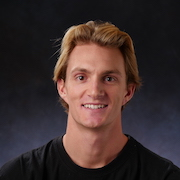
\includegraphics{PicOfMatt.JPG}
\caption{This is Matt Lawson before he cut his hair.}
\end{figure}

\begin{itemize}
\item
  By analyzing data, I would like to know how stoplights cycles could be
  improved to diminish traffic.
\item
  Six months after graduation, I would like to be traveling around the
  world. I am planning on graduating December 2020, so maybe somewhere
  in Europe or Asia. 5 years after that, I plan to be working as a data
  scientist somewhere. I don't really know or care where at this point,
  but I think it would be cool to work in a different country
  (especially Germany) for a while.
\item
  During my carreer, I hope to be able to have a significant positive
  impact on the environment. Hopefully I can do this with data science.
  In this course, I am hoping to learn how to use different tools that
  will allow me to analyzie many different types of data and draw corret
  conclusions about said data.
\item
  Also, I like to snowboard, hike, swim, and, as of recently, play
  poker.
\end{itemize}

\begin{center}\rule{0.5\linewidth}{\linethickness}\end{center}

\paragraph{Brandon Bowen}\label{brandon-bowen}

\begin{itemize}
\item
  I'm interested in the growing popularity of profesional gaming. Even
  now some profesional gamers are making the same amount as profesional
  sports player. How will this trend contiune? Will it eventualy become
  a world wide ``sport?''
\item
  Six months after graduation, I would at least want a stable job that I
  can work at for a couple of years before pursuing higher education.
  After 5 years if I already finished my higher education I would like
  to work in a foreign country such as Japan. Reason being i'm
  interested in the country of Japan itself and i'm also learning
  Japanese.
\item
  What I would want for my greatest career acomplishment to be is to be
  as successful as I can. In all honestly I don't know what my career
  holds for me therefore I can only strive to do the best I can in my
  field of work.
\item
  With these goals in mind, what I plan to take away from this course is
  R programing, interpreting data and finding conclusions for said data
  and combing all these skills to effictley gather, transform and
  communicate my data and work.
\item
  Something about me is I love to read on my off time with no specific
  genre in mind. Also i'm a competive gamer, while not profesional I do
  participate in a couple online tournaments and even in person
  tournaments.
\end{itemize}

\begin{center}\rule{0.5\linewidth}{\linethickness}\end{center}

\paragraph{Bing Mitchell}\label{bing-mitchell}

\begin{figure}
\centering
\includegraphics{PicOfBing.jpg}
\caption{Bing in Hawaii}
\end{figure}

\begin{itemize}
\item
  I want to be able to find insights about the game of Basketball by
  analyzing data.
\item
  6 Months after graduation, I would love to be travelling the world
  because I love to be in new places. 5 years after graduation, I would
  like to be a data analyst for a proffesional sports franchise
\end{itemize}

-I am hoping to be able to learn how to analyze data better, figure out
what is relevant and what isn't, and be able to put together nice
statistical reports

-I am from Piedmont, California which is right next to Oakland. I am a
Golden State Warriors fan and follow the NBA very closely.


\end{document}
